It is no secret that, in the last three years, \textit{Large Language Models} (LLMs) have fundamentally transformed our relationship with technology.
Their impact rivals the most significant innovations of the past century, such as the internet and the smartphone. When people contemplate \textit{Artificial Intelligence} (AI) today, they immediately think of ChatGPT or Claude, which have seamlessly integrated into our daily routines.
Yet these powerful tools come with significant environmental concerns. Their development and operation consume vast amounts of energy and water resource: modern data centers supporting these models require extensive cooling systems and electricity consumption that can rival small cities.

The computational complexity of these systems necessitates cloud-based deployment, which not only amplifies their environmental footprint but also fundamentally restricts user autonomy. This cloud dependency creates a concerning power dynamic where users have limited control over their tools, while simultaneously enabling extensive data collection practices and potential surveillance mechanisms that would be impossible with local, user-controlled alternatives.

In this more conversational opening chapter we will briefly examine the environmental and social impact of LLMs while highlighting the growing imperative for efficient, locally-deployable models that democratize access without depleting our planet's resources. Afterwards, we will outline the scope of this project, which aims to explore the potential of compression techniques to make LLMs more efficient.

The future of AI depends not just on what these models can do, but how sustainably they can do it.

\section{The social impact of LLMs}
The widespread adoption of LLMs has created ripple effects across virtually every sector of society, fundamentally altering how we work, learn, and create. In education, these tools have sparked heated debates about academic integrity while simultaneously offering new possibilities for personalized learning and accessibility for students with disabilities \cite{academic_integrity}. The workplace has experienced perhaps the most dramatic shifts, with entire professions grappling with automation anxiety while others discover unprecedented productivity gains. Creative industries find themselves in particularly complex territory: writers, artists, and content creators must navigate between leveraging AI as a collaborative tool and protecting their intellectual property from being absorbed into training datasets without consent or compensation \cite{artistic_integrity}.

Perhaps what is most striking is how these models have democratized access to sophisticated capabilities that were once the exclusive domain of experts. A small business owner can now generate marketing copy that rivals professional agencies, students can receive tutoring in subjects where human expertise might be scarce, and non-programmers can write functional code with natural language instructions. Yet this democratization comes with a troubling caveat: it's entirely dependent on maintaining access to centralized, corporate-controlled systems. When OpenAI experiences an outage, millions of users worldwide suddenly lose access to tools they've integrated into their daily workflows. When pricing models change, entire business models built around AI assistance can become unsustainable overnight.

This dependency becomes even more concerning when we consider the data these systems collect. Every interaction, every query, every creative prompt may potentially become part of these companies' datasets, raising questions about privacy and intellectual property.
As such, the need for transparency and user control over these systems has never been more urgent, and many believe that the future of AI must prioritize local, user-deployable models that empower individuals rather than centralizing power in the hands of a few corporations.

\section{The environmental impact of LLMs}

The computational demands of modern LLMs create an environmental footprint that grows exponentially with model size and usage. Training GPT-3, for instance, consumed an estimated 1,287 MWh of electricity, which is enough to power an average American home for over a century \cite{gpt_energy}. However, training represents only the tip of the iceberg; the real environmental cost lies in inference, where billions of daily queries across millions of users create a continuous drain on global energy resources. A recent study by Jegham et al. \cite{hungry_ai} estimates that OpenAI's GPT-4.5 requires ~6.7 Wh of energy for a medium sized query (i.e. 100 input tokens, and outputting 300 tokens) to be processed. This figure grows to ~20.5 Wh for a larger query (i.e. 1000 input tokens, and outputting 1000 tokens). To put this into perspective, this is equal to charging an average 40 Wh laptop battery to 50\%. A graph comparing the energy consumption of different LLMs with different prompt sizes is shown in Figure \ref{fig:energy_consumption}.

Data centers housing these models consume approximately 1-2\% of global electricity, a figure that's projected to reach 8\% by 2030 if current trends continue \cite{datacenter_energy}. The infrastructure supporting a single large-scale LLM requires thousands of high-performance GPUs running 24/7, each consuming as much power as several households.

Water consumption presents an equally pressing concern that receives far less attention. Modern data centers require extensive cooling systems, with some facilities consuming millions of gallons daily. According to their sustainability report \cite{google_report}, Google's water usage increased by ~20\% between 2021 and 2022, then by ~17\% from 2022 to 2023, and is largely attributed to AI inference operations \cite{ai_water}. In regions already facing water scarcity, this additional demand creates direct competition with human needs and agricultural requirements.

On the other hand, one has to keep in mind the embedded carbon cost of the hardware itself. Each GPU cluster supporting LLM operations represents significant emissions from manufacturing, shipping, and eventual disposal. The rapid pace of AI advancement drives frequent hardware upgrades, creating electronic waste streams that the recycling industry struggles to process effectively.

These environmental costs scale directly with model size and usage frequency, creating a fundamental tension between AI capabilities and sustainability.

\begin{figure}[!ht]
    \centering
    \begin{subfigure}[b]{0.8\textwidth}
        \centering
        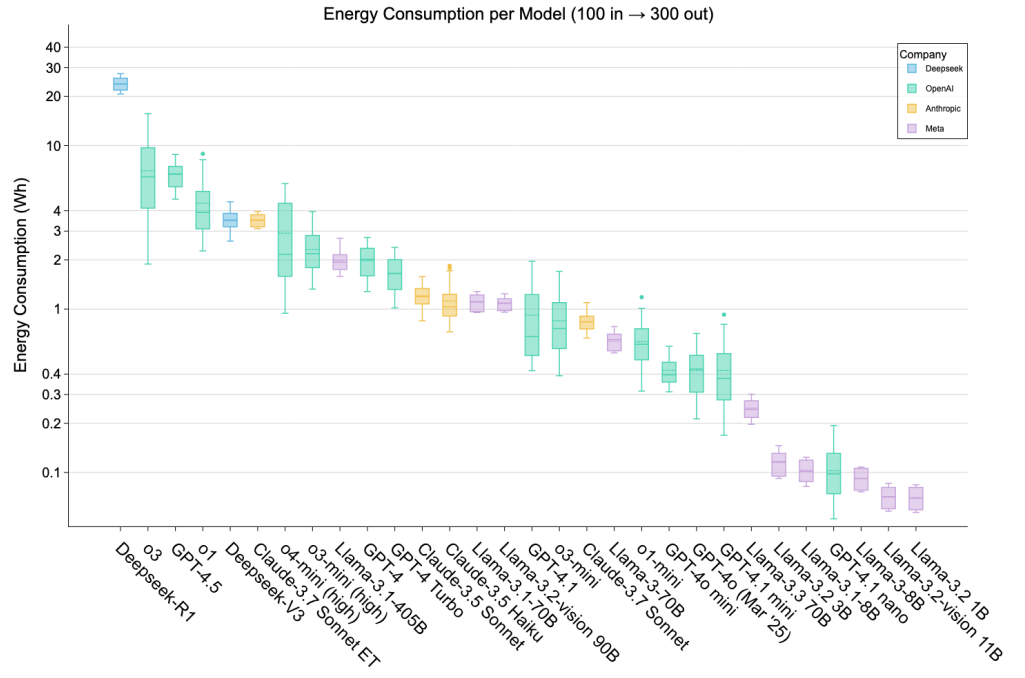
\includegraphics[width=\textwidth]{medium-size-consumption.png}
        \caption{Energy consumption for a small query (100 input tokens, 300 output tokens).}
        \label{fig:energy_consumption_small}
    \end{subfigure}
    \vskip 1em
    \begin{subfigure}[b]{0.8\textwidth}
        \centering
        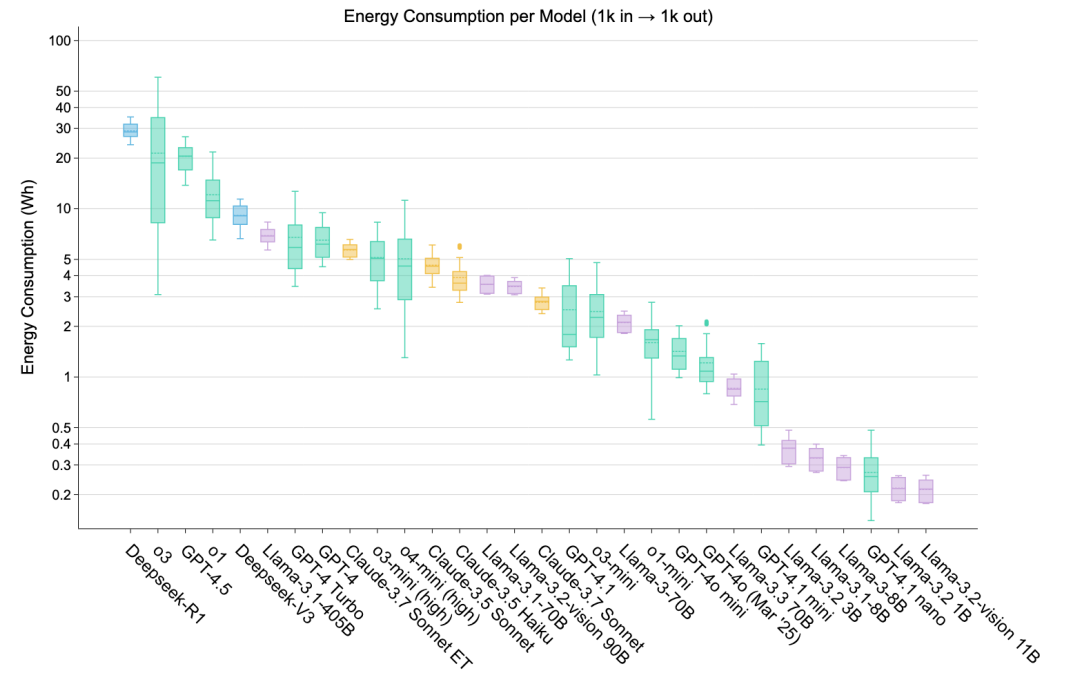
\includegraphics[width=\textwidth]{high-size-cosuption.png}
        \caption{Energy consumption for a large query (1000 input tokens, 1000 output tokens).}
        \label{fig:energy_consumption_large}
    \end{subfigure}
    \caption{Comparison of the energy consumption of different LLMs for small and large queries. The data highlights the significant increase in energy requirements as query size grows. These graphs have been sourced from \cite{hungry_ai}.}
    \label{fig:energy_consumption}
\end{figure}

\section{Scope}
While we've examined several critical challenges facing LLMs, it's worth emphasizing that these models hold significant potential for positive impact. As such, what was outlined in the previous sections points instead toward an urgent need for alternatives to the current paradigm of massive, centralized LLMs. A promising solution lies in compression techniques that can dramatically reduce model size while preserving core functionality. Through compression, billion-parameter server-sized models can be scaled down to more manageable ones that run much more efficiently.

\subsection{The main objective}
Given the context, the objective of this project is to push the boundaries of memory efficiency for small-scale LLMs by applying a targeted suite of compression techniques. We begin with a distilled model, a 1B parameter variant of LLaMA 3 \cite{llama3_1b}, which already represents a significantly reduced footprint compared to full-scale LLMs. From there, we explore and implement further optimizations, including depth and width pruning, \textit{Low-Rank Adaptation} (LoRA), and quantization.

Pruning allows us to remove redundant layers or neurons from the network architecture, trimming excess capacity without substantial loss of capability. Quantization reduces the bit-width of model weights and activations, decreasing both memory usage and compute requirements. LoRA, meanwhile, introduces a lightweight, parameter-efficient training mechanism that reduces the cost of fine-tuning and adaptation without (necessarily) modifying the base model weights. In this way, the model can be adapted to new tasks or domains with minimal overhead.

The reason behind the focus on maximizing memory efficiency is related to the fact that memory represents the most expensive constraint in our target deployment scenario, where the intended hardware platform consists of a low-power RISC-V SoC with severely constrained memory resources (further details on the target hardware can be found in Section \ref{target_hardware}). Crucially, optimizations that reduce memory footprint also translate directly into computational complexity improvements, creating a dual benefit for resource-constrained environments.

\subsection{How can optimization techniques help?}
Optimization techniques tackle the environmental, social, and infrastructure problems that come with large-scale LLMs. When models run more efficiently, they need far less power for each query. Smaller models can actually run on edge devices and other energy-efficient hardware, cutting down on electricity usage substantially. This efficiency boost also extends the useful life of older devices: hardware that might otherwise be considered obsolete can suddenly run modern LLMs, which helps reduce electronic waste and makes better use of existing resources.

There's also the autonomy angle. Compact models that run locally allows users to be independent from centralized servers when using AI. People can run LLMs right on their own devices without any internet connection, which means no data gets sent to third parties and there's no risk of surveillance. This approach supports decentralization and opens up AI access to areas with poor connectivity or limited economic resources.

In other words, optimization is a pathway toward environmentally sustainable, privacy-respecting, and widely accessible AI.


\section{Document structure}
Will write this when the document is finished.